% Four-symbol complete binary prefix code:
% a: 0 (1/2), b: 10 (1/4), c: 110 (1/8), d: 111 (1/8).
% Kraft: 1/2 + 1/4 + 1/8 + 1/8 = 1.
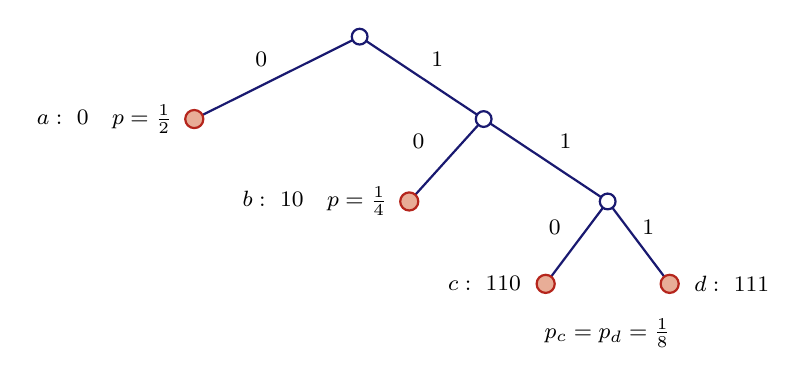
\begin{tikzpicture}[x=1.05cm,y=0.91cm,line cap=round]
  \tikzset{node/.style={circle,draw=MidnightBlue,fill=white,inner sep=0pt,
      minimum size=0.20cm,line width=0.8pt},
    leaf/.style={circle,draw=BrickRed,fill=BrickRed!30,inner sep=0pt,
      minimum size=0.23cm,line width=0.8pt}}
  \coordinate (root) at (0,0);
  \coordinate (a) at (-2,-1.15);
  \coordinate (r) at (1.5,-1.15);
  \coordinate (b) at (0.6,-2.3);
  \coordinate (s) at (3,-2.3);
  \coordinate (c) at (2.25,-3.45);
  \coordinate (d) at (3.75,-3.45);
  \draw[MidnightBlue,thick] (root)--(a) (root)--(r)
    (r)--(b) (r)--(s) (s)--(c) (s)--(d);
  \node[node] at (root) {};
  \node[leaf] at (a) {};
  \node[node] at (r) {};
  \node[leaf] at (b) {};
  \node[node] at (s) {};
  \node[leaf] at (c) {};
  \node[leaf] at (d) {};
  \node[font=\footnotesize,above left] at (-1, -0.55) {$0$};
  \node[font=\footnotesize,above right] at (0.75, -0.55) {$1$};
  \node[font=\footnotesize,above left] at (0.9, -1.7) {$0$};
  \node[font=\footnotesize,above right] at (2.3, -1.7) {$1$};
  \node[font=\footnotesize,above left] at (2.55, -2.9) {$0$};
  \node[font=\footnotesize,above right] at (3.3, -2.9) {$1$};
  \node[font=\footnotesize,anchor=east] at (-2.15,-1.15) {$a:\ 0\quad p=\frac12$};
  \node[font=\footnotesize,anchor=east] at (0.45,-2.3) {$b:\ 10\quad p=\frac14$};
  \node[font=\footnotesize,anchor=east] at (2.07,-3.45) {$c:\ 110$};
  \node[font=\footnotesize,anchor=west] at (3.93,-3.45) {$d:\ 111$};
  \node[font=\footnotesize,anchor=north] at (3,-3.8) {$p_c=p_d=\frac18$};
\end{tikzpicture}
